%!TEX root = /Users/dbreuer/Documents/Work/_FH/_Master/master_thesis/Main/Master Thesis.tex

\chapter{Prototypische Realisierung} % (fold)
\label{cha:prototypische_realisierung}

  Nachdem in das COSIMA-Projekt eingeführt und ein Szenario beschrieben wurde, dass zur Validierung der bisherigen Architektur dienen soll, wird in dem vorliegenden Kapitel die prototypische Realisierung der Architektur und des beschriebenen Szenario vorgestellt.
  
  In~\citep{handbuch_der_software_architektur} wird beschrieben, dass bei der Entwicklung von Rahmenwerken in der Regel zuvor eine Reihe von ähnlichen Anwendungen entstehen, aus denen dann die Gemeinsamkeiten in ein Rahmenwerk extrahiert werden. Da es sich bei COSIMA zum Teil auch um ein Rahmenwerk handelt ($\to$ \ref{sub:framework_oder_architektur}) hätte bei der Entwicklung entsprechend verfahren werden können. Auf Grund der beschrieben Neuartigkeit des Projekts wurde jedoch auf das beschriebene szenariobasierte Vorgehen ($\to$ \ref{cha:szenario}) zurückgegriffen.
  
  Da bis zu diesem Zeitpunkt die Architektur nur konzeptionell existierte, boten sich bei der Realisierung und Validierung zwei Vorgehensweisen:

  \begin{enumerate}[\slshape a)]
    \item Die Implementierung einer prototypischen Anwendung für das in \ref{sub:das_anwendungsszenario} beschriebene Szenario, bei gleichzeitiger Umsetzung der Architektur \emph{oder}
    \item Die prototypische Realisierung der Architektur anhand eines von dem Szenario unabhängigen Anwendungsfall und anschließende Implementierung der eigentlichen Anwendung auf Basis dieser so entstandenen Architektur.
  \end{enumerate}
  
  Da die zu entwickelnde Anwendung und die zugrunde liegende Architektur beziehungsweise das verwendete Rahmenwerk relativ unabhängig voneinander sind, ist Alternative \emph{a)} nur bedingt empfehlenswert. Eine Dekorrelation beider Aspekte ist, wie bereits zuvor festgestellt notwendig und zudem gängige Praxis. Aus diesem Grund wurde sich für Alternative \emph{b)} entschieden. Demzufolge ist eine Implementierung\footnote{Die Implementierung sowohl der Architektur als auch des Szenario sind in der Programmiersprache Java ($\to$ \url{http://java.sun.com/j2se/1.5.0/}) in Version 5.0 durchgeführt worden.} in zwei, voneinander unabhängigen Stufen vorgenommen worden:
  
  \begin{enumerate}
    \item Prototypische Realisierung der wesentlichen Architekturmerkmale anhand eines banalen Anwendungsfall \emph{und}
    \item Implementierung des in \ref{sub:das_anwendungsszenario} beschriebenen Szenario auf Basis dieser Architektur.
  \end{enumerate}
  
  Im ersten Abschnitt dieses Kapitel wird daher zunächst detailliert auf die Umsetzung der Architektur eingegangen. Im Anschluss daran findet sich eine Erläuterung zur Implementierung des Szenario. Die Validierung und deren Ergebnisse werden dann im Anschluss in Kapitel \ref{cha:validierung_der_architektur} dargelegt.

% - Vorgehen bei der Realisierung erläutern
% - Kurz (!!) auf das Santiago Projekt eingehen (da es im allerersten Schritt dazu gedient hat, eine erste funktionierende Grundlage der Architektur zu schaffen)
% - Wichtige Punkte herausarbeiten
% - Auf Implementierungsdetails nur an grundlegenden Stellen eingehen
% - Schwierigkeiten und vor allem deren Problemlösungen darstellen
% - Auswirkungen dieser Probleme/Lösungen für die Architektur
% - Fokus vor allem im Text auf das Vorgehen und Wendepunkte
% - Hauptteil der Quellcode
% - Funktionierenden Code mit Build Tool und Dokumentation ausliefern (!!)

\section{Realisierung der Architektur} % (fold)
\label{sec:realisierung_der_architektur}

  Bei dem gewählten \emph{bottom-up} Ansatz zur Entwicklung des Architekturprototypen musste zunächst ein geeigneter Anwendungsfall gefunden werden, der sich trotz einem Minimum an Komplexität dazu eignen musste, alle wesentlichen Architekturmerkmale extrahieren zu können. Zur besseren Kommunikation erhielt diese Anwendung den Codenamen \emph{Santiago} und ist formlos in Abbildung \ref{fig:images_Santiago_Anwendungsfall} strukturell dargestellt. Anhand der Abbildung lassen sich dann auch die drei wesentlichen Merkmale von Santiago leicht feststellen:

  \begin{figure}[!hb]
    \centering
      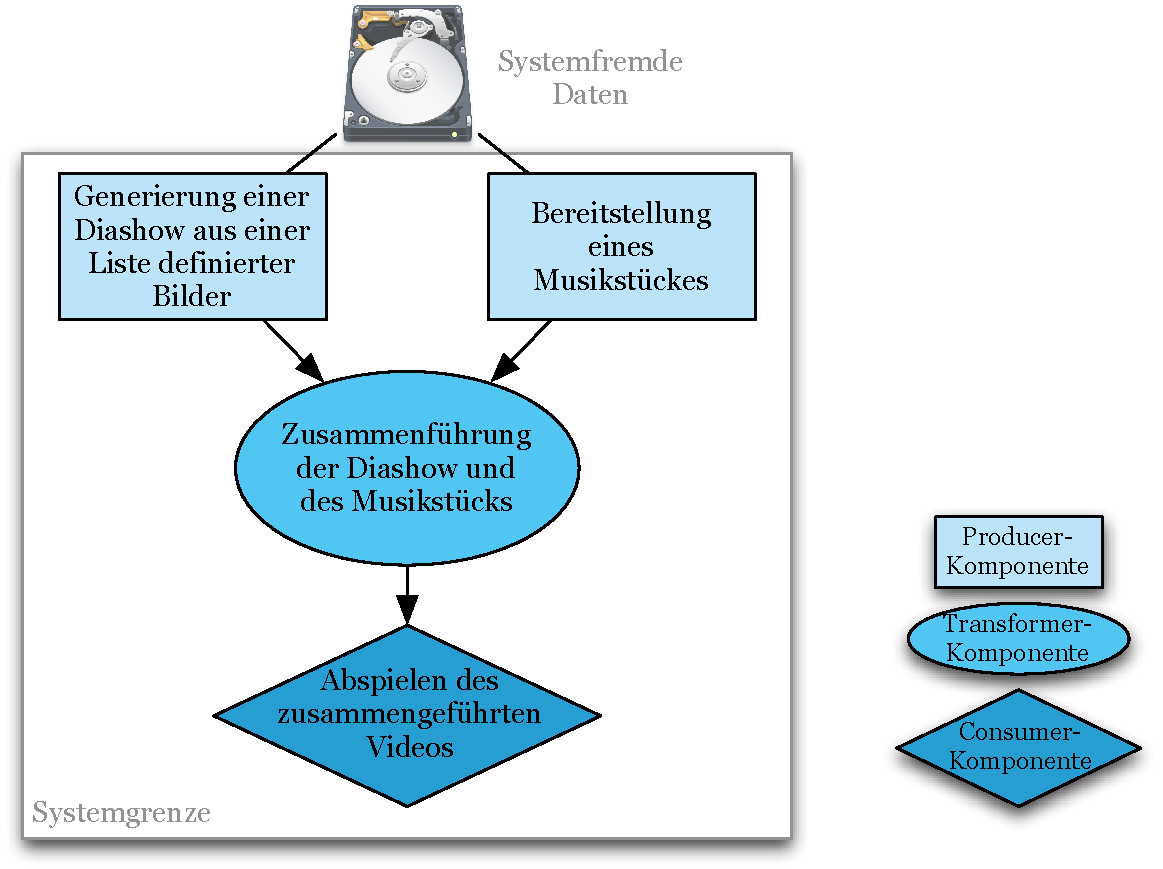
\includegraphics[width=.7\textwidth]{images/Santiago_Anwendungsfall.pdf}
    \caption{Anwendungsfall für die Realisierung der Architektur}
    \label{fig:images_Santiago_Anwendungsfall}
  \end{figure}
    
  \begin{itemize}
    \item Verarbeitung von unterschiedlichen Medien
    \item Umsetzung der einzelnen Verarbeitungsschritte in dedizierten Komponenten
    \item Anordnung dieser Komponenten nach dem Quelle-Komponente-Senke Prinzip
  \end{itemize}
  
  Trotz ihrer offensichtlichen Einfachheit konnte iterativ um diese Anwendung eine Architektur entwickelt werden, die alle notwendigen Charakteristika von COSIMA aufweist. Wie diese Entwicklung in den einzelnen Schritten im Detail aussah, beschreiben die folgenden Abschnitte.

  % TODO: Klären ob diese Punkte noch eingearbeitet werden müssen.
  % 
  % Beschreibung der Workflow Komponente. Vor allem Begründung warum selber gebaut -> Handelt es sich um Geschäftsprozesse? Dafür Prozess und Workflow definieren und auch auf Samma's Arbeit verweisen. Möglichkeiten zur Verwendung von BPEL aufzeigen.
  % 
  % Während der iterativen Entwicklung dieser Anwendung wurde sie sukzessive um die einzelnen Elemente und deren Funktionalitäten der COSIMA-Architektur ergänzt.
  % 
  % ZUR SERVICEKOMPOSITION: Aus den in~\ref{sub:service_komposition} genannten Gründen kann auch bei der prototypische Realisierung auf die Verwendung einer existierenden Prozessbeschreibungssprache verzichtet werden.
  
\subsection{Erste Schritte} % (fold)
\label{sub:erste_schritte}

  In der ersten Iteration wurde lediglich ein einfaches Programm geschrieben, dass sequentiell jede der einzelnen Operationen auf den Medien ausführt und in Listing \ref{lst:santiago_plain} dargestellt ist. Die einzelnen Operationen wurden dabei bereits in dedizierten Klassen gekapselt und über statische Methoden zugänglich gemacht. Der Kontrollfluss ist in dieser Implementierung implizit über Objektaufrufe realisiert und durch die Ausführungsreihenfolge konkret festgelegt. Der Datenfluss entsteht durch die Übergabe beziehungsweise Rückgabe von Objektinstanzen.

\lstinputlisting[caption=\texttt{SantiagoPlain}-Klasse zur einfachen Ausführung des Anwendungsfalls,label=lst:santiago_plain,language=Java,firstline=11,morekeywords={[2]VideoPlayer,SlideshowGenerator,MusicOMat}]{../code/Santiago/src/main/java/de/fhkoeln/santiago/codesamples/SantiagoPlain.java}

  Die rot markierten Klassen implementieren dabei die jeweiligen Operationen in geeigneter Weise\footnote{Ein Einblick in die Implementierung der einzelnen Klassen ist an dieser Stelle nicht weiter relevant. Der vollständige Quellcode findet sich auf der Begleit-CD zu dieser Arbeit.}. Den Zugriff auf diese Operationen über Klassenmethoden zu realisieren eignet sich jedoch nicht für den Einsatz in verteilten Umgebungen: Eine parallele Verwendung ein und der selben Komponente wäre so nur schwer umsetzbar. In der nächsten Iteration war es daher notwendig, den Zugriff auf die Operationen über einzelne Instanzen zu implementieren. Gleichzeitig sollte die Benennung der Methoden unabhängig von der eigentlichen Funktionalität erfolgen. Dadurch wird zwar ein gewisser Grad an Lesbarkeit des Codes eingebüßt, jedoch gewinnt man ein deutliches höhres Maß an Austauschbarkeit. Die Umsetzung dieser beiden Anforderungen erfolgte über die Etablierung der abstrakten Oberklasse \verb!AbstractComponent! (siehe Listing \ref{lst:abstract_component_simple_class}), da alle Komponenten zwei wesentliche Gemeinsamkeiten aufweisen, \emph{a)} Die Übergabe von Eingabeparametern und \emph{b)} Die Ausführung der Operation unter Berücksichtigung dieser Parameter. Die Oberklasse definiert dabei drei Methoden: Die Methode \verb!setInput(String [] inputs)!, um die notwendigen Parameter zu setzen; Die Methode \verb!execute()! als nach außen sichtbare Schnittstelle, um die Operation zu starten und die Methode \verb!_execute()! in der die eigentliche Operation intern implementiert ist.
  
  \lstinputlisting[caption=Einfache \texttt{AbstractComponent}-Klasse,label=lst:abstract_component_simple_class,language=Java,firstline=8,morekeywords={[3]execute,getInput,setInput}]{../code/Santiago/src/main/java/de/fhkoeln/santiago/codesamples/AbstractComponent.java}
  
  Das ausführende Programm aus Listing \ref{lst:santiago_plain} kann nun die generalisierten Komponenten mit ihren homogenen Schnittstellen verwenden um die einzelnen Operationen anzustoßen. Die Änderungen der Anwendung sind dabei in Listing \ref{lst:santiago_plain_with_general_components} dargestellt. Als eine erste Abstraktion der Parameter dient in diesem Fall noch ein primitives String-Array, im weiteren Verlauf wird daraus ein vollständiges \emph{Value-Object}~\citep[S. 486]{fowler03peaa} entstehen. Die Implementierung der \verb!execute()!-Methode ist nach dem \emph{Template Method} Entwurfsmuster vorgenommen worden~\citep[325]{design_patterns}\footnote{In späteren Iterationen lassen sich so leicht Funktionalitäten hinzufügen, die vor oder nach der eigentlichen Operation durchgeführt werden müssen.}.

  \lstinputlisting[caption=Erweitertes Santiago Programm mit generalisierten Komponenten,label=lst:santiago_plain_with_general_components,language=Java,firstline=21,lastline=34,morekeywords={[3]AbstractComponent}]{../code/Santiago/src/main/java/de/fhkoeln/santiago/codesamples/SantiagoPlainWithGeneralComponents.java}
  
  Für die nächste Iteration war es notwendig, wie bereits in Abbildung \ref{fig:schema_des_anwendungsszenario} dargestellt, dass eine Producer-Komponente das Musikstück erst innerhalb der Systemgrenzen \emph{bekannt machen} muss. Der Grund dafür ist, dass innerhalb einer COSIMA-Anwendung eine Transformer-Komponente nur Mediendaten verarbeiten kann, die bereits im System vorhanden sind, also über den Medien Broker abgerufen werden können. Im Kontext von COSIMA hat das die Bedeutung, dass ein Medienobjekt erzeugt und über den Medien Broker bereitgestellt wird. Für die Santiago Anwendung bedeutet es momentan lediglich, dass das String-Objekt \verb!musicPath! durch eine Instanz der \verb!MusicProvider!-Klasse (siehe Listing \ref{lst:santiago_plain_with_music_provider}) dem String-Objekt \verb!music! zugewiesen wird.
  
  \lstinputlisting[caption=Integration einer dedizierter Komponente zur Bereitstellung der Musik,label=lst:santiago_plain_with_music_provider,language=Java,firstline=21,lastline=24,morekeywords={[3]MusicProvider}]{../code/Santiago/src/main/java/de/fhkoeln/santiago/codesamples/SantiagoPlainWithMusicProvider.java}
  
  Dabei ist natürlich zu beachten, dass der \verb!MusicOMat!-Instanz nicht länger die Referenz auf das \verb!musicPath!-Objekt, sondern auf das \verb!music!-Objekt übergeben wird.
  
  Nachdem die notwendigen Komponenten zur Medienverarbeitung implementiert wurden, musste in der nächsten Iteration der Kontrollfluss über eine deklarative Beschreibung anzugeben sein. Des Weiteren musste diese Beschreibung durch eine dedizierte Komponente analysiert und ausgeführt werden. Die Entwicklung dieser Ablaufbeschreibung und ihrer ausführenden Instanz wird im folgenden Abschnitt näher beschrieben.
  
% subsection erste_schritte (end)
  
\subsection{Einführung einer deklarativen Ablaufbeschreibung} % (fold)
\label{sub:einfuehrung_einer_deklarativen_ablaufbeschreibung}

  Dafür folgende Schritte notwendig:
 
 - Definition einer Schnittstelle für Ausführung der Funktionalität\\
 - Einführung eines Value-Objects, zum Handling der Ein- und Ausgabedaten
 
  Anschließend Möglichkeit zur abstrakten (deklarativen) Definition der Ausführung notwendig (Workflow-Definition). Für den Prototypen wurde eine einfache Lösung selbst implementiert. Ermöglicht einen besseren Einblick in die Anforderungen und besseres Verständnis im Rahmen der Validierung. Verwendung einer etablierten Lösung wie BPEL hätte eine zusätzliche Komplexität eingeführt, die nicht zur Zielerreichung beigesteuert hätte (vgl. Umfang bei~\citep{samma08}). Auch ist keine zustandbasierte Lösung implementiert worden, wie sie bei~\citep{biornstad2006cfs} vorgeschlagen (und auch von BPEL implementiert). Grund: Ohnehin nur Prototyp, Inhalt weiterer Arbeiten.
  
\lstinputlisting[caption=\texttt{WorkflowDefinition}-Schnittstelle,label=lst:workflow_definition_interface,language=Java,firstline=12]{../code/COSIMA/src/main/java/de/fhkoeln/cosima/workflow/WorkflowDefinition.java}

\lstinputlisting[caption=Implementierung der \texttt{WorkflowDefinitionIterator}-Klasse,label=lst:workflow_definition_iterator,language=Java,firstline=12]{../code/COSIMA/src/main/java/de/fhkoeln/cosima/workflow/WorkflowDefinitionIterator.java}
% subsection einfuewhrung_einer_deklarativen_ablaufbeschreibung (end)
  
\subsection{Probleme und Lösungen} % (fold)
\label{sub:probleme_und_loesungen_architektur}

  - Welche Probleme sind aufgetaucht?
  - Wie wurden diese gelöst?
  - Auswirkungen auf die Architektur!
  - Workflow ohne externes Messaging System möglich!?

% subsection probleme_und_loesungen_architektur (end)

% section realisierung_der_architektur (end)

\section{Realisierung des Szenario} % (fold)
\label{sec:realisierung_des_szenario}

  - Nerstrand Projekt
  - wichtige Punkte beschreiben
  - top-down Ansatz

\subsection{Extrahierte Anforderungen} % (fold)
\label{sub:extrahierte_anforderungen}

% subsection extrahierte_anforderungen (end)

\subsection{Vorgehen} % (fold)
\label{sub:vorgehen_szenario}

  - wie wurde bei der Umsetzung des Anwendungsszenario vorgegangen?

% subsection vorgehen_szenario (end)

\subsection{Probleme und Lösungen} % (fold)
\label{sub:probleme_und_loesungen_szenario}

  - Welche Probleme sind aufgetaucht?
  - Wie wurden diese gelöst?
  - Auswirkungen auf die Architektur!

% subsection probleme_und_loesungen_szenario (end)

% section realisierung_des_szenario (end)

% chapter prototypische_realisierung (end)